\section{Equational reasoning}

\begin{frame}
    \frametitle{Now what?}

    We have a \alert{sound and complete} semantics for circuits as
    \alert{stream functions}.

    \wait

    But reasoning with streams can be a \alert{pain}...

    \wait
    Why not reason \alert{equationally}?
\end{frame}
\begin{frame}
    \frametitle{The two types of equation}

    \centering
    \begin{minipage}{0.49\textwidth}
        \centering
        \alert{Global}

        \vspace{1.5em}

        \dsptikzfig{strings/structure/cartesian/naturality-copy-lhs}[F][seq]
        =
        \dsptikzfig{strings/structure/cartesian/naturality-copy-rhs}[F][seq]
    \end{minipage}
    \begin{minipage}{0.49\textwidth}
        \centering
        \alert{Local}

        \vspace{1.5em}

        \dsptikzfig{circuits/axioms/fork-lhs}[v]
        =
        \dsptikzfig{circuits/axioms/fork-rhs}[v]
    \end{minipage}

    \vspace{1.5em}

    We want to stick to local equations \alert{as much as possible}.

\end{frame}

\begin{frame}
    \frametitle{What do the values do?}

    \centering
    \begin{minipage}{0.32\textwidth}
        \begin{equation*}
            \dsptikzfig{circuits/axioms/gate-lhs}
            =
            \dsptikzfig{circuits/axioms/gate-rhs-simple}
        \end{equation*}

        \visible<3->{
            \begin{equation*}
                \dsptikzfig{circuits/axioms/join-lhs}[v][w]
                =
                \dsptikzfig{circuits/axioms/join-rhs}[v][w]
            \end{equation*}
        }
    \end{minipage}
    \begin{minipage}{0.32\textwidth}
        \visible<2->{
            \begin{equation*}
                \dsptikzfig{circuits/axioms/fork-lhs}[v]
                =
                \dsptikzfig{circuits/axioms/fork-rhs}[v]
            \end{equation*}
        }

        \visible<4->{
            \begin{equation*}
                \dsptikzfig{circuits/axioms/stub-lhs}[v]
                =
                \dsptikzfig{strings/monoidal/empty}
            \end{equation*}
        }
    \end{minipage}
    \begin{minipage}{0.32\textwidth}
        \visible<5->{
            \begin{equation*}
                \dsptikzfig{circuits/axioms/disconnect-lhs}
                =
                \dsptikzfig{circuits/axioms/disconnect-rhs}
            \end{equation*}
        }
    \end{minipage}

    \wait

    \visible<6->{
        \begin{theorem}
            For \(
                \dsptikzfig{circuits/components/values/v}[\overline{v}]
            \) and \(
                \dsptikzfig{strings/category/f}[F][comb]
            \), there exists \(
                \dsptikzfig{circuits/components/values/v}[\overline{w}]
            \) such that \(
                \dsptikzfig{circuits/components/circuits/f-applied}[F][comb][\overline{v}]
                    =
                \dsptikzfig{circuits/components/values/v}[\overline{w}]
            \).
        \end{theorem}
    }
\end{frame}
\begin{frame}
    \frametitle{Let's get structural}

    \centering
    \wait

    \[(
        \dsptikzfig{strings/structure/monoid/merge}[comb],
        \dsptikzfig{strings/structure/monoid/init}[comb],
        \dsptikzfig{strings/structure/comonoid/copy}[comb],
        \dsptikzfig{strings/structure/comonoid/discard}[comb],
    )\] is a \alert{bialgebra}.

    \wait

    \begin{minipage}{0.21\textwidth}
        \begin{equation*}
            \iltikzfig{strings/structure/monoid/unitality-l-lhs}
            =
            \iltikzfig{strings/structure/monoid/unitality-l-rhs}
        \end{equation*}
    \end{minipage}
    \begin{minipage}{0.26\textwidth}
        \begin{equation*}
            \iltikzfig{strings/structure/monoid/associativity-lhs}
            =
            \iltikzfig{strings/structure/monoid/associativity-rhs}
        \end{equation*}
    \end{minipage}
    \begin{minipage}{0.26\textwidth}
        \begin{equation*}
            \iltikzfig{strings/structure/monoid/commutativity-lhs}
            =
            \iltikzfig{strings/structure/monoid/commutativity-rhs}
        \end{equation*}
    \end{minipage}

    \begin{minipage}{0.21\textwidth}
        \begin{equation*}
            \iltikzfig{strings/structure/comonoid/unitality-l-lhs}
            =
            \iltikzfig{strings/structure/comonoid/unitality-l-rhs}
        \end{equation*}
    \end{minipage}
    \begin{minipage}{0.26\textwidth}
        \begin{equation*}
            \iltikzfig{strings/structure/comonoid/associativity-lhs}
            =
            \iltikzfig{strings/structure/comonoid/associativity-rhs}
        \end{equation*}
    \end{minipage}
    \begin{minipage}{0.26\textwidth}
        \begin{equation*}
            \iltikzfig{strings/structure/comonoid/commutativity-lhs}
            =
            \iltikzfig{strings/structure/comonoid/commutativity-rhs}
        \end{equation*}
    \end{minipage}

    \begin{minipage}{0.28\textwidth}
        \begin{equation*}
            \iltikzfig{strings/structure/bialgebra/merge-copy-lhs}
            =
            \iltikzfig{strings/structure/bialgebra/merge-copy-rhs}
        \end{equation*}
    \end{minipage}
    \begin{minipage}{0.23\textwidth}
        \begin{equation*}
            \iltikzfig{strings/structure/bialgebra/init-copy-lhs}
            =
            \iltikzfig{strings/structure/bialgebra/init-copy-rhs}
        \end{equation*}
    \end{minipage}
    \begin{minipage}{0.23\textwidth}
        \begin{equation*}
            \iltikzfig{strings/structure/bialgebra/merge-discard-lhs}
            =
            \iltikzfig{strings/structure/bialgebra/merge-discard-rhs}
        \end{equation*}
    \end{minipage}
    \begin{minipage}{0.2\textwidth}
        \begin{equation*}
            \iltikzfig{strings/structure/bialgebra/init-discard-lhs}
            =
            \iltikzfig{strings/structure/bialgebra/init-discard-rhs}
        \end{equation*}
    \end{minipage}
\end{frame}
\begin{frame}
    \frametitle{Splitting things up}

    To deal with more complicated circuits we need to \alert{isolate} the
    sequential and combinational components...

    \centering
    \wait
    \[
        \dsptikzfig{strings/category/f}[F][seq]
        =
        \dsptikzfig{circuits/productivity/pre-mealy-form}[F][s]
    \]

    \wait
    This is \emph{almost} another Mealy machine moment...
    \raisebox{1.5em}{
        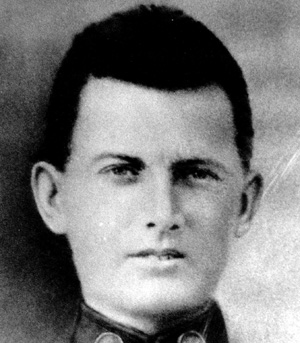
\includegraphics[width=0.1\textwidth]{imgs/mealy}
    }

\end{frame}
\begin{frame}
    \frametitle{Getting rid of non-delay-guarded feedback}

    Instant feedback

\end{frame}
\begin{frame}
    \frametitle{Let's get structural}

    What more structure can we add?

    Cartesian

\end{frame}
\begin{frame}
    \frametitle{Let's get structural}

    Unfolding

\end{frame}
\begin{frame}
    \frametitle{Running the simulation}

    \centering
    \begin{equation*}
        \dsptikzfig{circuits/productivity/productive-goal-lhs-verbose}[F][v]
        =
        \dsptikzfig{circuits/productivity/productive-goal-rhs-verbose}[G][w]
    \end{equation*}

\end{frame}
\begin{frame}
    \frametitle{Running the simulation}

    First the \emph{combinational} case...

    \centering
    \begin{equation*}
        \dsptikzfig{circuits/axioms/streaming-lhs-verbose}
        =
        \dsptikzfig{circuits/axioms/streaming-rhs}
    \end{equation*}

\end{frame}
\begin{frame}
    \frametitle{Working it all out}

    Full reduction

\end{frame}
